\section{La economía descentralizada}

Este capítulo tiene como objetivo entender cómo se ordena una economía descentralizada, es decir, una economía donde los agentes toman decisiones de manera privada. Para esto tomaremos como principal eje un modelo Walrsaiano, el cual es de equilibrio general, la gracia del modelo radica en que a diferencia de los modelos de equilibrio parcial los precios de equilibrio se determinan considerando dos o más mercados. Por tanto, el equilibrio en algún mercado afecta al equilibrio de los demás mercados. 

Los mecanismos en los cuales los agentes toman sus decisiones y llegan a un punto eficiente determinado nos llevará a definir dos teoremas del bienestar, los cuales reflejan distintas maneras de abordar la distribución de recursos en una economía. 

\subsection{Motivación del Modelo de Equilibrio General}

Para definir los modelos de equilibrio general partiendo de base en los modelos de equilibrio parcial conviene dar un pequeño repaso de estos. Uno de los economistas que definió el paradigma en el cual se basan los modelos de equilibrio parcial fue \textbf{Alfred Marshall},\marginnote{\textbf{Alfred Marshall:} Economista británico que durante finales del siglo XIX, conocido por ser fundador de la escuela neoclásica. Su visión marginalista de la economía influye las bases de la economía hasta día de hoy.}[-4cm] el cual popularizó el uso de las curvas de oferta y demanda como herramientas para la determinación de precios. Los modelos de equilibrio parcial buscan describir la determinación de precios bajo oferta y demanda de un mercado específico tratando el resto de la economía como constante. Para dar contexto, si analizaramos el mercado de autos importados supondríamos que los ajustes en este mercado no tienen efectos sobre mercados relacionados. Por ejemplo, el modelo predice cómo afecta un arancel al precio de los autos importados, pero no aborda los efectos del arancel sobre la demanda y producción de autos producidos domésticamente.\footnote{El mercado de autos importados se considera un mercado distinto al mercado de autos producidos domésticamente.}

El modelo de equilibrio parcial es de gran utilidad para modelar efectos de distintas políticas sobre el precio y bienestar de los agentes en un mercado en específico. En la realidad sin embargo, como distintos mercados están interactuando constantemente un shock en uno de ellos puede derivar a múltiples ajustes en mercados relacionados. Volviendo al ejemplo anterior, este arancel por autos importados podría llevar a un aumento de ventas de autos domésticos al ser bienes sustitutos. 

En resumen, el \textbf{modelo de equilibrio general}\marginnote{\textbf{Modelo de Equilibrio General:} Modelo económico que busca explicar la determinación de precios dentro de una economía con dos o más mercados.}[-3cm] describe dos o más mercados relacionados que se ajustan a la vez y entre ellos. Analizar el equilibrio de un número arbitrario de mercados es complejo, por suerte limitarnos a dos mercados y plantear ciertos supuestos nos permite extraer las conclusiones que encontramos relevantes para esta ocasión. 

\subsection{Introducción del modelo Walrasiano}

Describiremos los supuestos y sustancia del modelo, el mecanismo por el cual se llega al equilibrio. El Modelo Walrasiano como indica su nombre es producto del trabajo de \textbf{León Walras}\marginnote{\textbf{León Walras:} Economista francés de la escuela (neoclásica) de Lausana. Considerado fundador de la economía matemática.}[0cm]. En este modelo trataremos un economía con un número de bienes y agentes finitos basada en el intercambio, es decir, no hay dinero sino que los individuos intercambian bienes los cuales se les dota de manera exógena. Entonces la riqueza del individuo se determina por el valor de la dotación de bienes que posea.\footnote{Un paso anterior es la producción de estos bienes, pero no conviene referirse a ese aspecto aún.}

Por lo tanto el problema de los individuos $i$ será maximizar su utilidad $u(\cdot)$ demandando bienes $x$ de un total de $N$ bienes sujeto a su riqueza siendo la dotación inicial $e$  y precios.
\begin{align*}
    \max_{x \in \mathbb{R}^N_+}u^i (x) \quad \text{s.a} \quad p\cdot x \leq p\cdot e^i
\end{align*}
De esta manera es que los invididuos demandan los bienes y se determinan los precios: en el \textbf{Equilibrio Walrasiano} será el vector de tamaño $1\times N$ de precios y consumo de bienes tales que (i) los individuos maximizan su utilidad sujeto a su riqueza, (ii) la demanda total de un bien es igual a la dotación total del bien.

Estando o no estando en equilibrio el modelo sigue la \textbf{Ley de Walras}\marginnote{\textbf{Ley de Walras:} La suma del valor del excedente de deamanda de todos los mercados es igual a cero.}[0cm], la cual indica que suma del valor del exceso de demanda de todos los mercados es igual a cero. Entiéndase exceso de demanda positiva como que en un mercado la demanda por un bien excede la producción/dotación de este, consecuentemente un exceso de demanda negativo implica que hay más unidades de las que se demandan. Esto tiene dos importantes resultados.
\begin{itemize}
    \item Si hay un exceso de demanda positiva en un mercado significa que hay un exceso de demanda negativa en otro mercado. Es decir, si un mercado está en desequilibrio otro mercado debe estar en desequilibrio.
    \item Si $n-1$ mercados están en equilibrio, el $n-$ésimo mercado también estará en equilibrio. 
\end{itemize}
Este último resultado nos permite limitarnos a dos mercados para simplificar la resolución del modelo.

Un aspecto crucial del modelo es el \textbf{criterio de Pareto}.\marginnote{\textbf{Criterio de Pareto:}}[0cm] Los individuos comercian sus bienes con otros individuos, es intuitivo entender que un individuo solo intercambiará una cantidad de un bien mientras que el bien que le llegue a cambio le genere una utilidad mayor, es decir, solo accederan a intercambiar si son más felices con el acuerdo. Por lo tanto, habrá un punto en que dejarán de intercambiarse puesto que se agotaron todas las transacciones posibles, en este equilibrio ninguno de los dos puede estar mejor sin perjudicar al otro. Puesto en otras palabras: a medida que hayan intercambios que sean \textbf{mejorías de pareto}\marginnote{\textbf{Mejorías de Pareto:}}[-2cm] se tomarán hasta llegar a un \textbf{óptimo de Pareto}.\marginnote{\textbf{Óptimo de Pareto:}}[0cm] Estos conceptos se definiran luego.

Por último, algunos supuestos implíticos y explícitos del modelo son:
\begin{enumerate}
    \item No hay poder de mercado, los dos agentes en la economía serán tomadores de precios. 
    \item Información completa. Los dos individuos están al tanto de los bienes que hay en la economía, su cantidad y utilidad que les proporciona tanto a el como al otro. 
    \item No hay costos de transacción. 
    \item No hay externalidades. El consumo de un bien no afecta la utilidad de un externo de ninguna manera.\footnote{Este supuesto se puede levantar y llevar al mismo resultado de equilibrio bajo ciertas condiciones, asumiremos que no existe tal posibilidad.} 
\end{enumerate}

Ahora describiremos el modelo en más detalle asumiendo que tendremos dos agentes y dos bienes. 

\subsection{Caja de Edgeworth}

La \textbf{Caja de Edgeworth}\marginnote{\textbf{Caja de Edgeworth:} Herramienta gráfica para representar un Modelo de Equilibrio Walrasiano.}[0cm] será la representación gráfica del modelo. Esta herramienta fue desarrollada por \textbf{Francis Edgeworth}\marginnote{\textbf{Francis Edgeworth:} Economista y estadístico británico que propone las curvas de indiferencia y caja de Edgeworth.}[3cm] y \textbf{Arthur Bowley},\marginnote{\textbf{Arthur Bowley:} Economista y estadístico británico pionero de usar técnicas de muestreo en encuestas sociales.}[6.5cm] economistas y estadísticos británicos. Las dimensiones de esta caja obedecerán a las dotaciones totales de cada bien, en esta misma podremos graficar las curvas de indiferencia de los individuos y demás conceptos que definiremos más adelante. 

Esta economía considera dos individuos $i \in A,B$ que se intercambian dos bienes $j \in x,y$. Las dotaciones de bienes que tenga cada individuo se puede describir como un vector $\in \mathbb{R}^2_+$, más precisamente las dotaciones para un individuo $i$ serán:
\begin{equation*}
    \omega_i = (\omega_{ix} , \omega_{iy}) \in \mathbb{R}^2_+
\end{equation*}
En la figura \ref{fig:caja dimensiones} podemos observar que las dimensiones de la caja son $\omega_x = \omega_{Ax} + \omega_{Bx}$ por un lado y $\omega_y = \omega_{Ay} + \omega_{By}$ por el otro. Donde además ubicamos la dotación inicial como un punto dentro de la caja $\omega^E \in \mathbb{R}^2_+$.
\begin{figure}
    \centering
    \caption{Dimensiones de la caja de Edgeworth}
    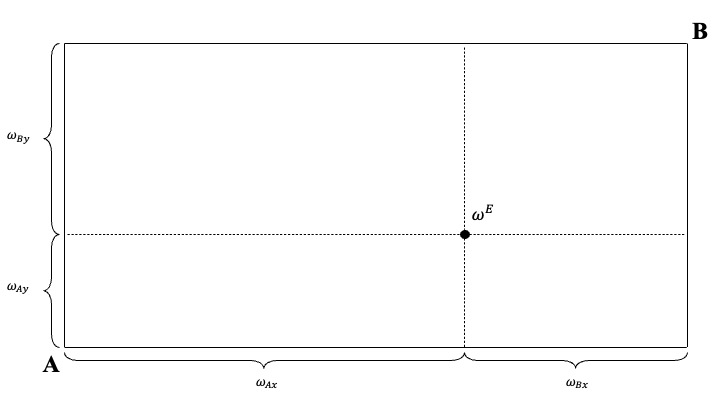
\includegraphics[width=\textwidth]{Figuras/EG Dotacion inicial.jpeg}
    \label{fig:caja dimensiones}
\end{figure}
Los mercados se encargarán de asignar precios a cada bien dadas las preferencias y dotaciones, estos precios los podemos denotar como un vector $p = (p_x, p_y) \in \mathbb{R}^2_+$. Para el individuo $i$ la riqueza se puede denotar como la cantidad de un bien ponderado por su precio: 
\begin{equation*}
    R_i = p_x \cdot \omega_{ix} + p_y \cdot \omega_{iy}
\end{equation*}
La riqueza será análogo a las restricción presupuestarias a la que está sujeta la maximización de utilidad. Es decir, el individuo $i$ maximizará su función de utilidad, en este caso del tipo Cobb-Douglas, consumiendo bienes $x,y$ y su restricción no estará activa mientras consuma menos o igual que su riqueza.
\begin{align*}
    \max_{x,y} &\quad u_i(x,y) = x_i^\alpha y_i^{\beta} \\
    \text{s.a.} &\quad R_i \leq p_x \cdot x_i + p_y \cdot y_i
\end{align*}
Se pueden graficar las curvas de indiferencia dada las preferencias de cada individuo dentro de la caja. Un hecho importante a recordar de las curvas de indiferencias es que curvas de indiferencias más a la derecha son mejores situaciones y lo contrario si nos movemos a la izquierda. Hay que considerar que dado que el individuo $B$ está desde otro punto de vista su curva de indiferencia es mejor mientras más a la izquierda esté.
\begin{figure}[htbp]
    \centering
    \caption{Curvas de indiferencia y lente de mejorías de pareto}
    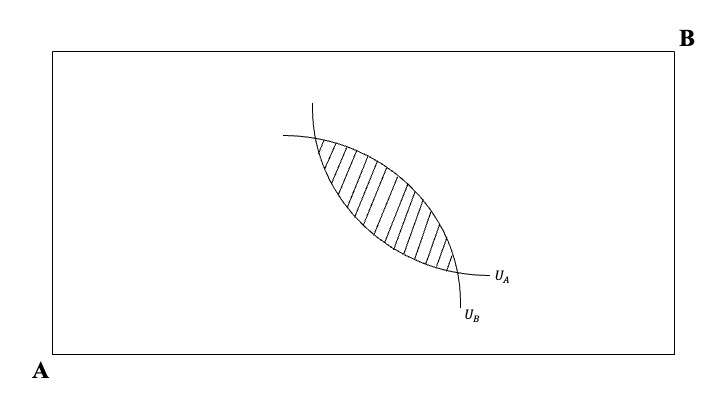
\includegraphics[width=\textwidth]{Figuras/EG Curvas de indiferencias.jpeg}
    \label{fig:caja indiferencias}
\end{figure}

\subsection{Eficiencia y óptimos de pareto}

Dadas las preferencias y dotaciones los individuos podrán intercambiar bienes para maximizar su utilidad. Este proceso puede ser visto desde el punto de vista del criterio de Pareto, paradigma acuñado por \textbf{Vilfredo Pareto}.\marginnote{\textbf{Vilfredo Pareto:} Economista italiano, adopta los equilibrios walrasianos e incorporó a ellos el concepto de óptimo de Pareto.}[-7cm] En este contexto un intercambio que aumenta la utilidad de al menos uno y no perjudica la utilidad del otro sería una \textbf{mejoría de pareto}\marginnote{\textbf{Mejoría de Pareto:} Transición en donde al menos un individuo esté en una mejor posición sin perjudicar a otro.}[-4cm]. El punto en donde se acaban las oportunidades de intercambio será el \textbf{óptimo de Pareto}\marginnote{\textbf{Óptimo de Pareto:} Punto en donde todas las mejorías de Pareto posibles se han agotado.}[-1cm]. Podemos encontrar graficamente los puntos de mejoría de pareto el lente de mejorías de pareto, el cual es el área rayada en la figura \ref{fig:caja indiferencias}.

Algunos detalles a aclarar de estos conceptos pueden ser los siguientes.
Estar en un óptimo de pareto no es sinónimo perfecto de estar en Equilibrio Walrasiano, el punto eficiente de pareto tan solo describe una situación en donde no hay intercambios \textit{win-win} posibles. También cabe mencionar que un punto eficiente no necesariamente es deseable bajo otros criterios: Una dotación inicial donde $A$ ó $B$ concentra todos los recursos es un punto eficiente bajo criterio de Pareto.

Una manera de encontrar un punto óptimo de Pareto es igualar las \textbf{tasas marginales de sustitución}\marginnote{\textbf{Tasa Marginal de Sustitución:} Unidades de un bien que se están dispuestos a renunciar por una unidad marginal del otro bien, manteniendo el mismo nivel de utilidad.}[-1.5cm] de bienes de los individuos (condición \ref{eq:TMS=TMS}). Esto tiene sentido intuitivo dado que en un punto óptimo de Pareto ningun individuo está dispuesto a intercambiar sus bienes puesto que no aumentarían su utilidad. Por ejemplo, si el individuo $A$ está más dispuesto a intercambiar bienes $x$ que $B$ el cual está más dispuesto a intercambiar sus bienes $y$, entonces habrá una mejoría de Pareto posible del intercambio. En dicha situación la disposición de intercambiar cada bien es diferente para cada individuo por lo que tiene sentido intercambiar. Gráficamente veríamos como en el óptimo las curvas de indiferencia de ambos individuos son tangentes.
\begin{equation}
    TMS_{x,y}^A = TMS_{x,y}^B \label{eq:TMS=TMS}
\end{equation}
La tasa marginal se calcula como la derivada parcial de la utilidad respecto a un bien divido por la derivada parcial de la utilidad respecto al otro bien. Por lo que podemos redefinir la condición \ref{eq:TMS=TMS} como: 
\begin{align*}
    \frac{    \frac{\partial u_A(x,y)}{\partial x}       }{      \frac{\partial u_A(x,y)}{\partial y}     } & =  \frac{    \frac{\partial u_B(x,y)}{\partial x}       }{      \frac{\partial u_B(x,y)}{\partial y}     } 
\end{align*}
La \textbf{curva de contrato} es la colección de puntos óptimos de pareto dentro de la caja de Edgeworth.\marginnote{\textbf{Curva de contrato:} Colección de puntos óptimos de Pareto dentro de la caja de Edgeworth.} A continuación llegamos a la expresión que denotan todos los óptimos de pareto que componen la curva de contrato para los individuos $A$ y $B$. Siendo que el problema para $A$ se plantea como:
\begin{align*}
    \max_{x,y} &\quad u_A(x,y) = x_A^\alpha y_A^{\beta}\quad \\
    \text{s.a.} &\quad p_x \cdot w_{Ax} + p_y \cdot w_{Ay} = p_x \cdot x_A + p_y \cdot y_A
\end{align*}
El problema para $B$ es simétrico:\footnote{Cada vez que un problema sea simétrico significa que la solución algebráica seguirá el mismo proceso, por lo que podemos ocupar el resultado de un individuo para obtener directamente el resultado del otro sin hacer el proceso de optimización de nuevo.}
\begin{align*}
    \max_{x,y} &\quad u_B(x,y) = x_B^\alpha y_B^{\beta}\quad \\
    \text{s.a.} &\quad p_x \cdot w_{Bx} + p_y \cdot w_{By} = p_x \cdot x_B + p_y \cdot y_B
\end{align*}
Derivamos para obtener la expresión de la tasa marginal de sustitución para ambos individuos. 
\begin{align*}
    TMS_A  = \frac{\alpha x_A^{\alpha -1} y_A^{\beta}}{\beta x_A^\alpha y_A^{\beta -1} } = \frac{\alpha}{\beta} \cdot \frac{y_A}{x_A} \\
    TMS_B= \frac{\alpha x_B^{\alpha -1} y_B^{\beta}}{\beta x_B^\alpha y_B^{\beta -1} } = \frac{\alpha}{\beta} \cdot \frac{y_B}{x_B} 
\end{align*}
Igualamos tasas marginales de sustitución,
\begin{align*}
    TMS_A = TMS_B \quad \Longrightarrow \quad& \frac{\alpha}{\beta} \cdot \frac{y_A}{x_A} = \frac{\alpha}{\beta} \cdot \frac{y_B}{x_B} \\
   &  \frac{y_A}{x_A} = \frac{y_B}{x_B}
\end{align*}
Es directo entender que la suma de los bienes de cada individuo será el total de bienes en la economía,
\begin{align*}
    x_A + x_B = \omega_x \quad 
    y_A + y_B = \omega_y
\end{align*}
Y por tanto aprovechamos para definir nuestra curva de contrato Reemplazando una de aquellas en la expresión anterior.
\begin{align*}
    \frac{y_A}{x_A} &= \frac{\omega_y - y_A}{\omega_x - x_A} \\
    y_A\omega_x &= x_A\omega_y
\end{align*}
Reordenando la expresión,
\begin{equation}
    x_A \cdot \left( \frac{\omega_y}{ \omega_x} \right) = y_A \label{eq:curva de contrato}
\end{equation}
\begin{figure}[htbp]
    \centering
    \caption{Curva de contrato}
    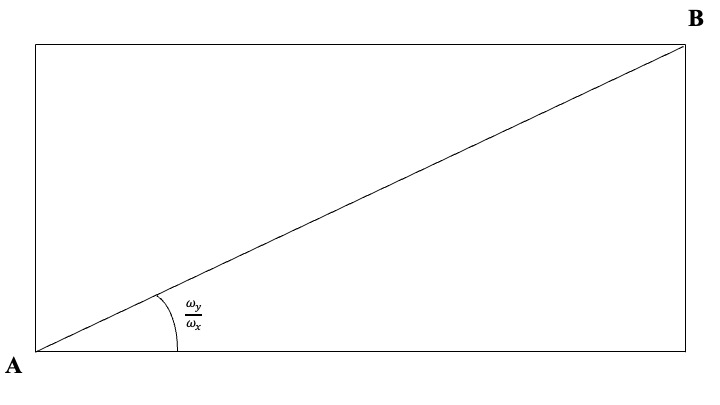
\includegraphics[width=\textwidth]{Figuras/EG Curva de contrato.jpeg}
    \label{fig:diapositiva3}
\end{figure}
Es decir, una dotación que cumpla con la expresión \ref{eq:curva de contrato} pertenece a la curva de contrato y por ende es óptimo de Pareto, se agotaron las posibilidades de intercambio por lo que no se puede aumentar la utilidad de uno sin reducir la del otro. La curva de contrato va a tener diferentes formas dependiendo de la función de utilidad de los individuos, en algunos casos no habrá.\footnote{Tarea para el anexo.} 

\subsection{Demandas Marshallianas}

Los individuos tendrán una \textbf{demanda marshalliana}\marginnote{\textbf{Demandas Marshallianas:} Son las demandas óptimas resultantes de un problema de maximización sujeto a alguna restricción.} acorde a sus preferencias y riqueza. Si resolvemos el problema para A encontraremos la demanda del individuo para cada bien. En este caso diremos que $\alpha,\beta >0$ y que $1 - \alpha = \beta $
\begin{align*}
    \max_{x,y} &\quad u_A(x,y) = x_A^\alpha y_A^{\beta}\quad \\
    \text{s.a.} &\quad R_A = p_x \cdot x_A + p_y \cdot y_A
\end{align*}
Planteando el lagrangeano,
\begin{equation*}
    \mathcal{L}= x_A^\alpha y_A^{\beta} + \lambda (R_A - p_x \cdot x_A - p_y \cdot y_A)
\end{equation*}
Derivamos las condiciones de primer orden.
\begin{align*}
    \frac{\partial \mathcal{L}}{\partial x_A} = \alpha x_A^{\alpha-1}y_A^\beta - \lambda_x p_x = 0 \quad \quad
    \frac{\partial \mathcal{L}}{\partial y_A} = \beta x_A^\alpha y_A^{\beta -1} - \lambda_y p_y = 0
\end{align*}
Se despejan los lambdas y se igualan las expresiones.
\begin{align*}
    & \lambda_x = \frac{\alpha x_A^{\alpha-1}y_A^\beta }{p_x} \quad 
    \lambda_y = \frac{\beta x_A^\alpha y_A^{\beta-1}}{p_y} \longrightarrow \frac{\alpha x_A^{\alpha-1}y_A^\beta }{p_x} = \frac{\beta x_A^\alpha y_A^{\beta-1}}{p_y} \\
    \text{Reescribiendo,}\quad & x_A = y_A  \left( \frac{p_y \alpha}{p_x \beta} \right)  \quad y_A = x_A \left(  \frac{p_x \beta}{p_y\alpha}  \right)
\end{align*}
El siguiente paso es reemplazar alguna de las expresiones anteriores en la restricción:
\begin{align*}
    p_x\left( y_A\frac{p_y\alpha}{p_x\beta} \right) + p_yy_A = R_A
\end{align*}
Por lo tanto las demandas marshallianas de $A$ serán expresadas como:
\begin{align*}
    y_A^* = \frac{R_A}{p_y} \beta & \quad  x_A^* = \frac{R_A}{p_x} \alpha
\end{align*}
Como el problema es simétrico para $B$ podemos directamente decir:
\begin{align*}
    y_B^* = \frac{R_B}{p_y} \beta & \quad  x_B^* = \frac{R_B}{p_x} \alpha
\end{align*}
Las demandas marshallianas estarán en función de la riqueza, el precio del bien y las preferencias.

\subsection{Precios relativos}

Los precios relativos en esta economía están determinados por la dotación y preferencias y serán tales que todos los mercados estén en equilibrio. Lo que importa no son los los valor nominal que se les da a los precios sino el precio de un bien en relación al otro, es por esto que un mismo equilibrio se puede sostener con un vector precios $p=(1,2)$ como con un vector $p=(2,4)$, si bien los valores cambiaron el segundo bien sigue siendo el doble de caro que el primero. 

Al resolver el modelo podemos normalizar uno de los precios a 1, de esta manera simplificamos el proceso. Esto es tener un precio numerario, si se tiene un vector de precios $p = (p_i,p_j)$ se multiplica por $1/p_i$, dejándolos como $p = (1, \frac{p_j}{p_i})$. La gracia está en que tanto la primera expresión del vector como la segunda funcionan para un mismo equilibrio.

Para obtener los precios relativos apelamos a la ley de Walras: la demanda total de un bien tiene que ser igual a la cantidad que existe.
\begin{equation*}
    x_A^* + x_B^* = \omega_x, \quad \quad y_A^* + y_B^* = \omega_y
\end{equation*}
Tomando el caso del bien $x$ reemplazamos las demandas marshallianas.
\begin{align*}
   \frac{R_A}{p_x} \alpha + \frac{R_B}{p_x} \alpha  &= \omega_x \\
   \frac{\alpha}{p_x} (R_A + R_B) &= \omega_x
\end{align*}
Despejando $p_x$ de esta expresión y (por simetría) expresando también $p_y$.
\begin{align*}
    p_x = (R_A + R_B)\frac{\alpha}{\omega_x}, \quad \quad p_y = (R_A + R_B)\frac{\beta}{\omega_y}
\end{align*}
Lo cual hace sentido, a mayor preferencia por determinado bien mayor es el precio, por otro lado a menor dotación del bien mayor su precio. Por convención diremos que la riqueza total se puede escribir como $R_A + R_B = R = p_x\omega_x + p_y\omega_y$. Dada esta expresión tendremos un problema, todavía no hemos despejado los precios puesto que estos dependen de la riqueza la cual depende recursivamente de los precios. Podemos hacer dos cosas, una de ellas es normalizar uno de los precios a 1, y la otra opción es dividir directamente $p_y/p_x$ para obtener $p_y$ en relación a $p_x$. 

Los precios relativos se pueden expresar entonces como:
\begin{align*}
    \frac{p_y}{p_x} = \frac{ \frac{R\alpha}{\omega_x}  }{  \frac{R\beta}{\omega_y}  } = \frac{\beta \omega_x}{\alpha \omega_y}
\end{align*} 

\subsection{Teoremas fundamentales de la economía del bienestar}

\textsc{Primer teorema del bienestar} 

\textbf{Todo Equilibrio Walrasiano es óptimo de Pareto}. Este teorema plantea que bajo igualdad en el equilibrio de oferta y demanda en los mercados no habrán oportunidades de intercambio.\footnote{Demostrado en Arrow, Kenneth J. and Gerard Debreu, “Existence of Equilibrium for a Competitive Economy,” Econometrica, 1954.} Este teorema se relaciona profundamente con las ideas más liberales de la economía, como la mano invisible, cada individuo buscando su propio beneficio llegaría a un punto eficiente para la economía en su conjunto. 

\textsc{Segundo teorema del bienestar} 

\textbf{Todo óptimo de Pareto puede conseguirse mediante un Equilibrio Walrasiano}. Este teorema abre a la posibilidlad de distribuir las dotaciones iniciales de manera de conseguir un Equilibrio Walrasiano deseado de manera eficiente. Este teorema se relaciona con las ideas redistributivas y de Estado de bienestar sin perder la eficiencia del mercado. 

\subsection{Equilibrio con producción}

Habiamos asumido en un inicio que hay una dotación de los bienes sin habernos metido en la producción de los mismos. Incluir la producción de los bienes es más que nada hacer un paso anterior donde la producción de bienes dependerá de la dotación de factores productivos.

Si le mata la curiosidad, el modelo de equilibrio de producción está en el anexo.

